\documentclass{standalone}
\usepackage{tikz}
\usetikzlibrary{shapes.geometric}
\begin{document}
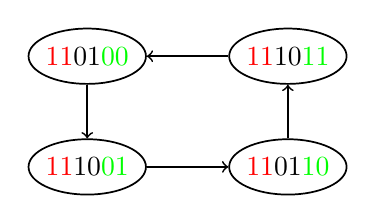
\begin{tikzpicture}
[every node/.style={inner sep=0pt}]
\node (1) [ellipse, minimum size=20.0pt, fill=white, line width=0.625pt, draw=black] at (37.5pt, -25.0pt) {\textcolor{red}{11}\textcolor{black}{01}\textcolor{green}{00}};
\node (2) [ellipse, minimum size=20.0pt, fill=white, line width=0.625pt, draw=black] at (37.5pt, -65.0pt) {\textcolor{red}{11}\textcolor{black}{10}\textcolor{green}{01}};
\node (3) [ellipse, minimum size=20.0pt, fill=white, line width=0.625pt, draw=black] at (110pt, -65.0pt) {\textcolor{red}{11}\textcolor{black}{01}\textcolor{green}{10}};
\node (4) [ellipse, minimum size=20.0pt, fill=white, line width=0.625pt, draw=black] at (110pt, -25.0pt) {\textcolor{red}{11}\textcolor{black}{10}\textcolor{green}{11}};
\draw [line width=0.625, ->, color=black] (1) to  (2);
\draw [line width=0.625, ->, color=black] (2) to  (3);
\draw [line width=0.625, ->, color=black] (3) to  (4);
\draw [line width=0.625, ->, color=black] (4) to  (1);
\end{tikzpicture}

\end{document}
